\documentclass{article}
\usepackage[utf8]{inputenc}
\usepackage{pythontex}
\usepackage[a4paper, margin=2cm]{geometry}
\usepackage{graphicx}
\usepackage{booktabs}


\begin{document}
\begin{center}
\section*{Predicting risk of drug consumption based on personality features, demographic variables and previous consumption.}

\begin{pycode}
print(f"Camila Batista Rahal and Elena Maestre Soteras")
\end{pycode}
\end{center}

\subsection*{Abstract}
Drug consumption and misuse remain significant public health concerns, shaped by an interaction of personality traits, demographic characteristics, and historical behavior. The study employs a variety of predictive models (logistic regression, lasso, random forest, and Xgboost) to analyze the relationships between this personality factors, demographic variables, and drug consumption patterns, aiming to identify significant predictors for the risk of future drug use. The participants were classified as 'consumer' or 'non-consumer.' XGBoost baseline achieve the best performance with a recall of 84.3\%, followed by Random Forest with recall of 83\%. Random Forest achieves the highest AUC (0.90), making it the most effective model for distinguishing between consumers and non-consumers classes. Bagging Classifier and Optimized Random Forest closely follow with an AUC of 0.89, indicating strong performance with balanced sensitivity and specificity. This research demonstrates the potential of data-driven methods for understanding and addressing drug use behaviors, while offering a foundation for future studies that integrate psychological and demographic data.



\subsection*{Exploratory Data Analysis}
The dataset had 1,885 participants, no missing data, and the features were quantified and standardized. The dataset shows a high prevalence of participants aged 18–24, a predominance of consumers within this group, a disproportionate number of White participants compared to other ethnicities, and a higher number of male consumers than female (Table 1). Summary statistics (Table 2) confirm key predictors like age, country, ethnicity, impulsivity, and sensation-seeking. Lower education appears linked to higher use. Target imbalance (mean = 0.552) was handled with SMOTE. Figure 1 below visualizes the distribution of drug usage frequencies across various substances. It highlights trends such as a large number of participants reporting never having used heroin or crack, while substances like ecstasy and mushrooms show relatively higher recent use. Additionally, there is a high prevalence of users for substances like chocolate, nicotine, caffeine, alcohol, and cannabis. These substances were excluded when creating the target variable.

\begin{figure}[h!]
    \centering
    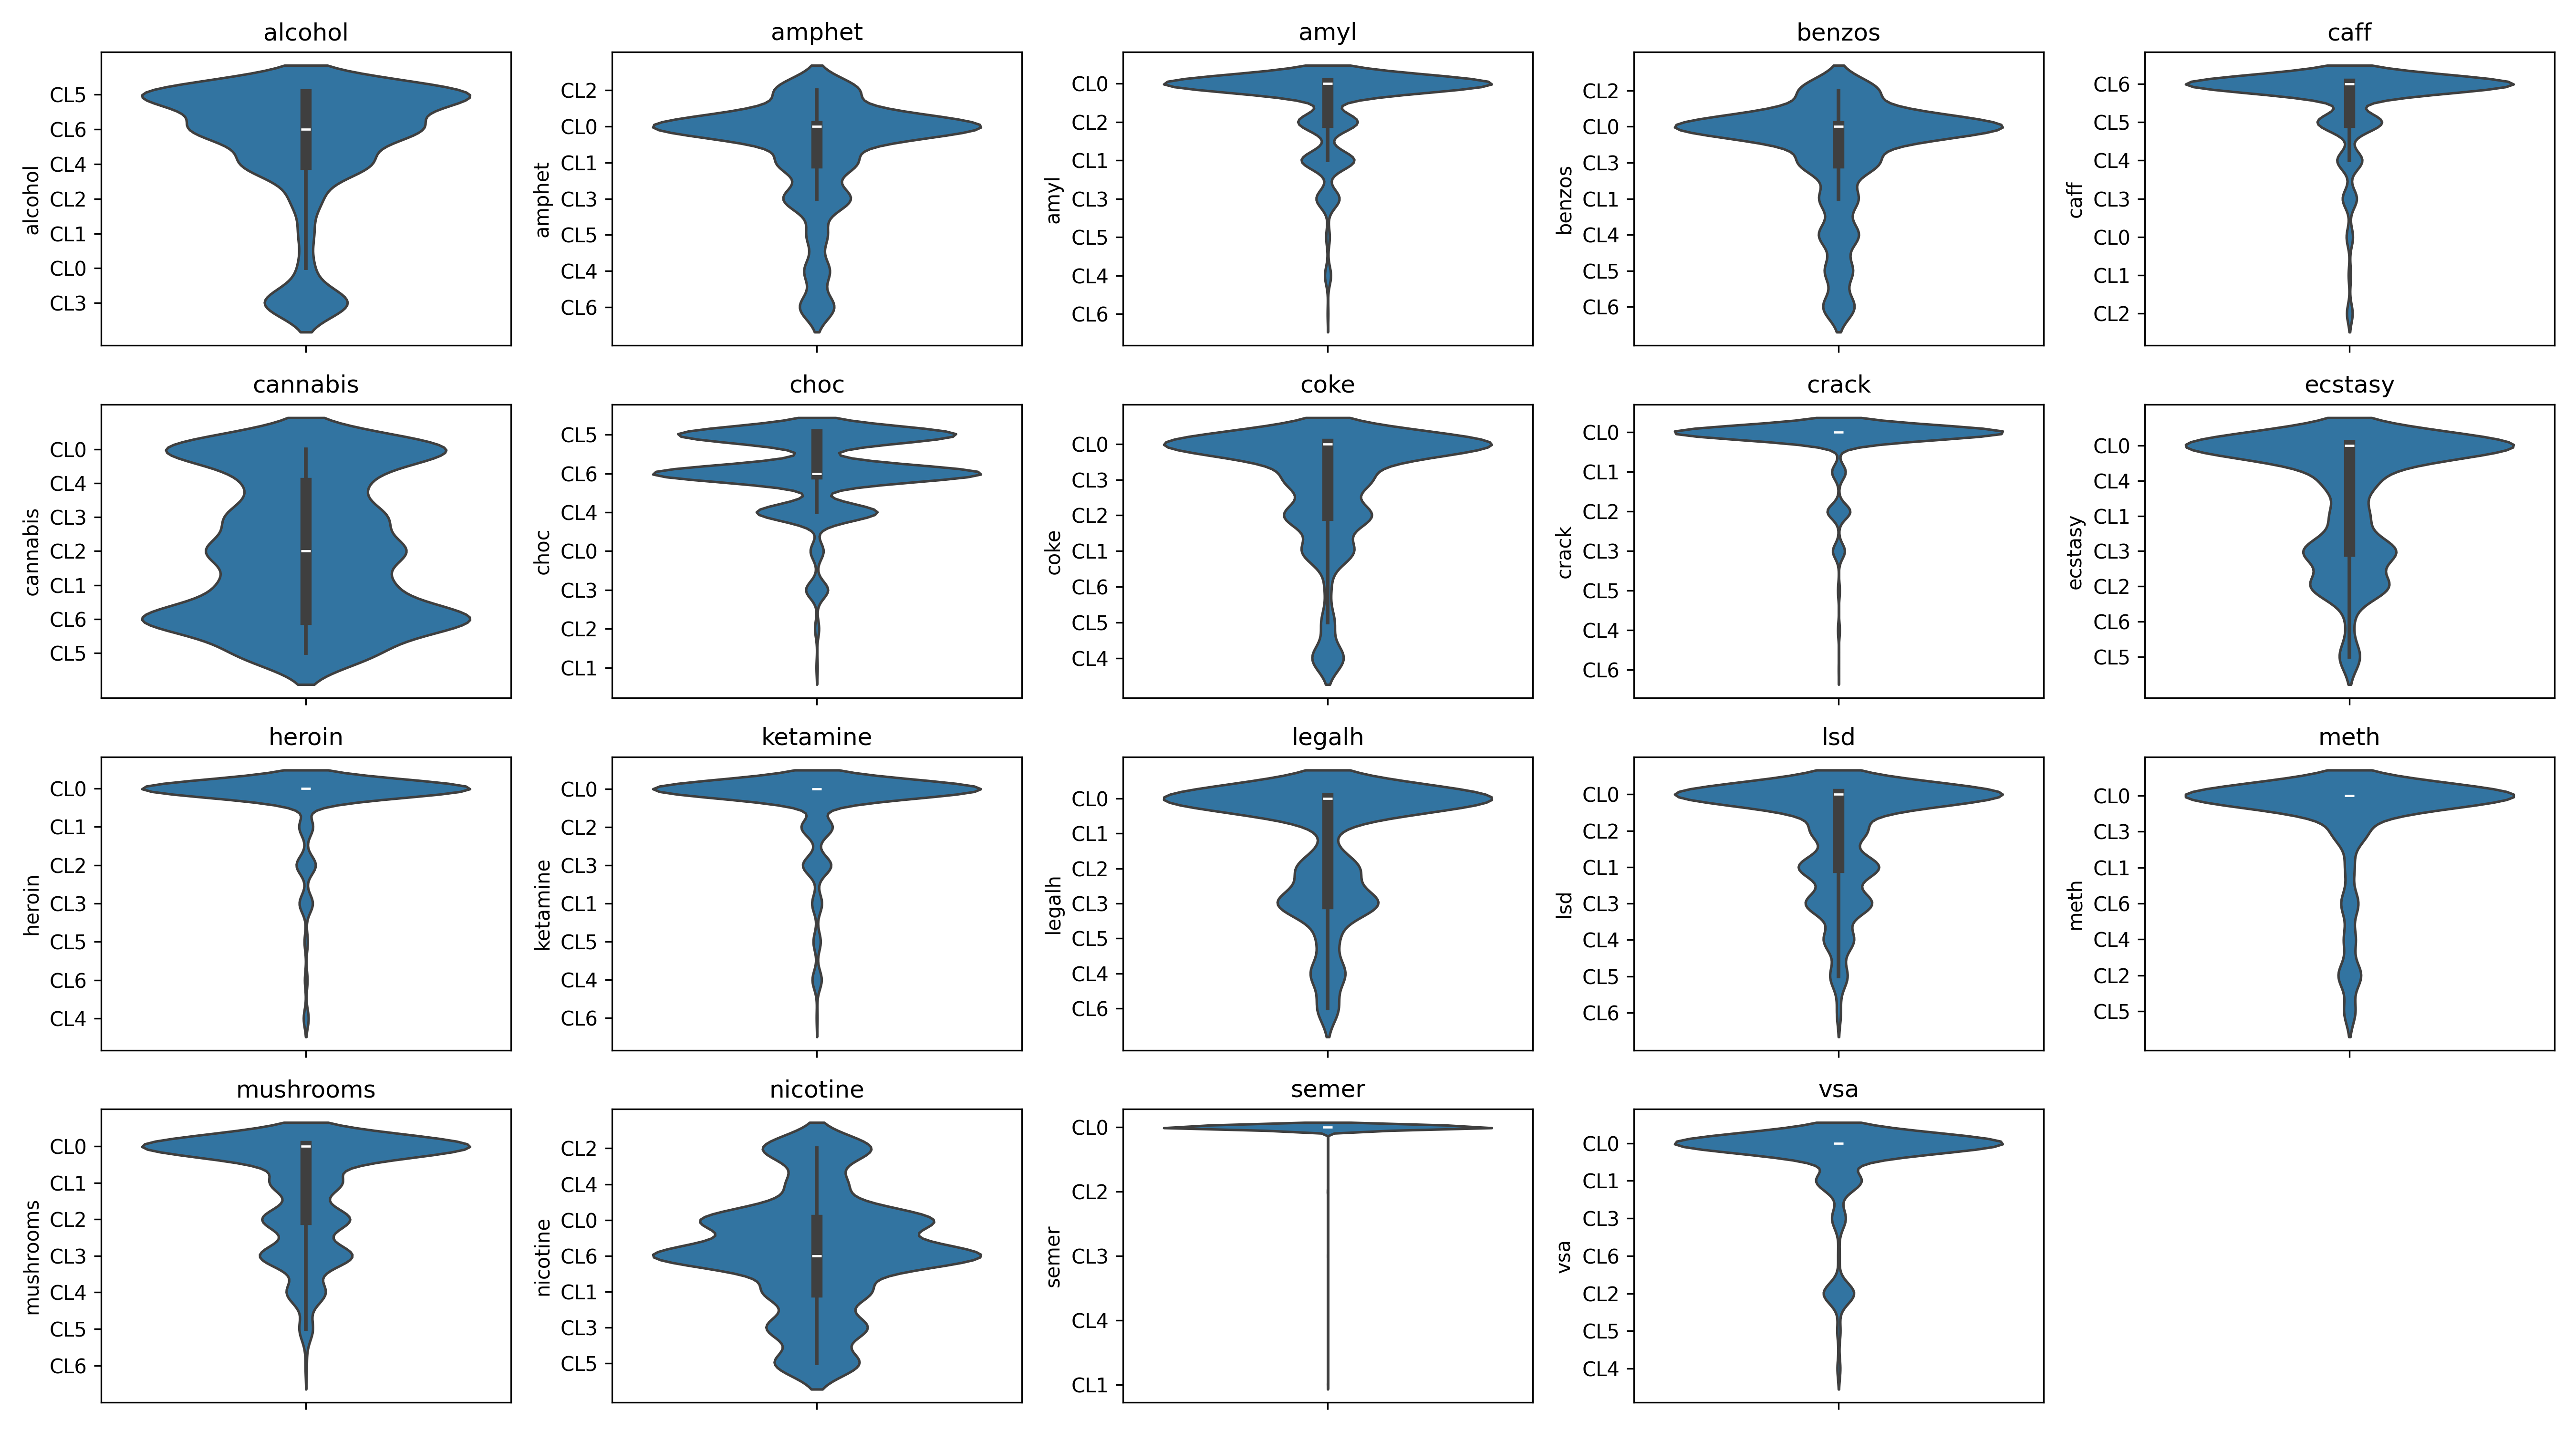
\includegraphics[width=\textwidth]{violin_plots_all_columns.png}
    \caption{Violin plot of all drugs consuming behavior from CL0 (Never used) to CL6 (Used last day).}
    \label{fig:violin_plot}
\end{figure}

\begin{figure}[h!]
    \centering
    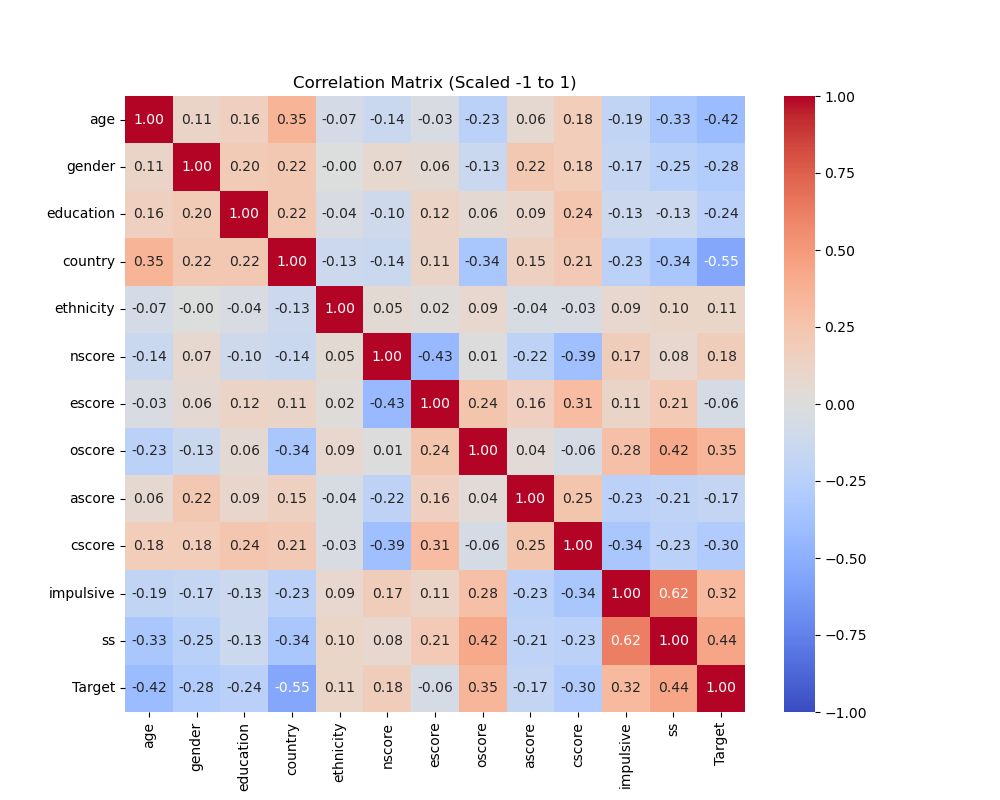
\includegraphics[width=\textwidth]{correlation-matrixpng.png}
    \caption{Correlation matrix of features.}
    \label{fig:correlation-matrix}
\end{figure}

To analyze the correlation between features a correlation matrix was performed (Figure 2). It demonstrated that "Country" and "Age" show strong negative correlations with the target (-0.55 and -0.42), while "Sensation-Seeking" (ss) and "Impulsivity" have positive correlations (0.44 and 0.32), indicating their influence on user classification. Additionally, "nscore" and "escore" are moderately negatively correlated (-0.43), and "ss" and "Impulsive" are strongly positively correlated (0.62), suggesting feature interdependencies. This analysis hints the most important features it can be used as a predictor for the model.


\subsection*{Data Preparation}

\begin{itemize}
    \item Data used was preprocessed previously.
    \item 5\% of the data was reserved as final evaluation set *Hold-Out, and the remaining data was split into 80\% training, 10\% validation, 10\% testing. Random seeds ensured reproducibility.
    \item Target was binary (consumer vs non-consumer) and 11 features: the Big Five personality traits (NEO-FFI-R), those are nscore (Neutoticism), escore (Extraversion), oscore (Openness to Experience), ascore (Agreeableness), and cscore (Conscientiousness). Impulsivity (BIS-11), sensation seeking (ImpSS), and demographic information: age, gender, education, and country.
    \item Data was standardized.
\end{itemize}

\subsubsection*{Models implemented}

\begin{itemize}
    \item Logistic Regression with L1 regularization
    \item Random Forest (baseline)
    \item Random Forest (Optimized with hyperparameters)
    \item XGBoost (baseline)
    \item XGBoost (Optimized with hyperparameters)
    \item SVM
    \item Decision Tree
    \item Bagging Classifier
\end{itemize}


\subsubsection*{Model evaluation metrics}

Each models performance was evaluated using, besides the validation and hold-out set, accuracy, precision and recall, f1 score, cross-validation *only on 3 models, and ROC-AUC.
In this project, which focuses on predicting the risk of drug consumption based on personality features, demographic variables, and previous consumption, the primary evaluation metric is recall. Recall is prioritized because the goal is to ensure that individuals who are actual consumers are accurately identified, minimizing false negatives. This is particularly important as missing potential consumers (false negatives) could lead to missed opportunities for intervention. While recall is the primary focus, precision is also monitored to ensure that the model maintains reasonable targeting, avoiding an excessive number of false positives. Additionally, F1-Score is used as a balanced metric to evaluate the trade-off between precision and recall, and ROC-AUC is included to assess the overall discriminatory power of the models.

\subsubsection*{Feature importance analysis}

\begin{itemize}
    \item \textbf{Logistic Regression with L1 regularization:} "ss" has the highest positive coefficient, while "age" has a significant negative coefficient, indicating their contrasting roles in prediction. Lasso excluded impulsiveness.
    
    \item \textbf{Linear SVM:} "ss" is the most significant positive predictor, "age" contributes negatively, others are smaller.
    
    \item \textbf{Bagging Classifier:} "Age" and "ss" dominate, age is strongest.
    
    \item \textbf{Decision Tree:} "Age" is dominant, followed by "ss".
    
    \item \textbf{Random Forest:} Both "ss" and "age" are key predictors.
    
    \item \textbf{Optimized XGBoost:} "Age" is top, followed by "ss".
    
    \item \textbf{Optimized Random Forest:} "ss" and "age" show balanced importance.
    
    \item \textbf{Conclusion:} "ss" and "age" are most important across models.
\end{itemize}

\subsection*{Results}

\subsubsection*{Model performance}

When focusing on recall, the Baseline XGBoost achieves the highest recall (84.3\%) followed by baseline Random Forest on the validation set, and the Bagging Classifier and Baseline XGBoost show the highest recall (80.7\%) on the hold-out set (Table 3). These results suggest that these models are particularly effective in identifying positive cases (consumers). The inconsistency of the results between the validation set and the hold-out, and the lower performance of the optimized models against the baseline models shows that there still space for improvement.

\subsubsection*{Cross-validation}
The evaluation used Stratified K-Fold Cross-Validation (5 folds) for Logistic Regression and during manual hyperparameter tuning for XGBoost, while GridSearchCV with 5-fold cross-validation was employed for the optimized Random Forest and the optimized XGBoost. 

Cross-Validation metrics for Logistic Regression with Lasso:
Mean Precision: 0.8128
Mean Recall: 0.7877
Mean F1 Score: 0.8000
Mean ROC-AUC: 0.8670

Cross-Validation metrics for Random Forest (Optimized):
Best cross-validation F1 score: 0.8062

Cross-Validation for XGBoost (Optimized):
Mean Logloss: 0.4471 ± 0.0276
Mean AUC: 0.8762 ± 0.0139

The result shows that XGBoost performs well, with accurate probability predictions (logloss: 0.4471) and strong class distinction (AUC: 0.8762), with consistent performance across folds (low standard deviations).


\subsubsection*{ROC AUC}

Random Forest achieved the highest AUC (0.90), followed by Bagging and Optimized Random Forest (0.89). Optimized XGBoost (0.88) outperformed its baseline (0.86). Logistic Regression and SVM showed solid results (0.86–0.87), while Decision Tree had the lowest AUC (0.85).

\begin{figure}[h!]
    \centering
    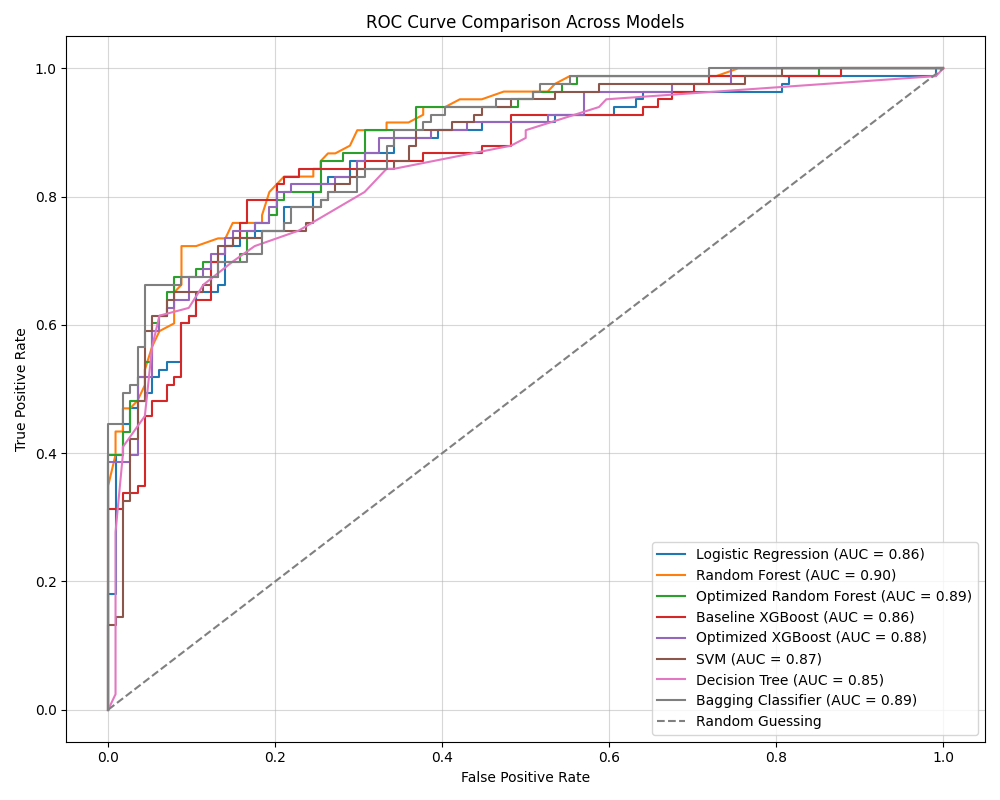
\includegraphics[width=\textwidth]{Figure_1.png}
    \caption{ROC Curve comparison across supervised machine learning models.}
    \label{fig:ROC}
\end{figure}

\subsection*{Discussion}

Model performance consistency suggests strong data patterns and stable predictors. Sensation seeking (ss) and age consistently emerged as the top predictors across models. Logistic Regression and SVM highlighted ss positively and age negatively. Tree-based models also emphasized these features, with Optimized XGBoost and Random Forest showing strong generalization. Despite existing evidence, Lasso excluded impulsivity, possibly due to multicollinearity or weak individual effect.

\subsubsection*{Implications}
Results support using psychological and demographic data for early risk identification in public health strategies.

\subsubsection*{Limitations}
The datasets imbalance and youth-skewed sample may limit generalizability. Broader, more diverse data is needed in future research. Excluding variables may have overlooked interactions between legal and illegal substances. The static nature of the data also omits temporal trends that could inform targeted interventions. Future studies should include older, more diverse populations and explore dynamic usage patterns for improved insight and model performance.

\subsection*{Conclusion}

This study demonstrates that personality traits—especially sensation seeking—and age are key predictors of psychoactive drug use, with models like XGBoost and Random Forest achieving strong performance. Integrating psychological and demographic data into predictive models offers valuable tools for early identification and targeted public health interventions.

\subsection*{Tables}
\begin{pycode}
print(r"\begin{table}[h!]")
print(r"\centering")
print(r"\small")
print(r"\caption{Demographics Summary}")
print(r"\label{tab:summary-demographic}")
print(r"\begin{tabular}{|l|r|r|}")
print(r"\hline")
print(r"\textbf{Target} & \textbf{Non-consumer} & \textbf{Consumer} \\ \hline")

# Age category
print(r"\multicolumn{3}{|l|}{\textbf{Age category}} \\ \hline")
age_data = [
    ("18-24 years", 113, 524),
    ("25-34 years", 218, 262),
    ("35-44 years", 215, 140),
    ("45-54 years", 211, 83),
    ("55-64 years", 70, 23),
    ("65+ years", 13, 5)
    ]
for row in age_data:
    print(f"{row[0]} & {row[1]} & {row[2]} \\\\ \hline")

# Gender category
print(r"\multicolumn{3}{|l|}{\textbf{Gender category}} \\ \hline")
gender_data = [
    ("Female", 552, 385),
    ("Male", 288, 652)
    ]
for row in gender_data:
    print(f"{row[0]} & {row[1]} & {row[2]} \\\\ \hline")

# Education category
print(r"\multicolumn{3}{|l|}{\textbf{Education category}} \\ \hline")
education_data = [
    ("Doctorate degree", 53, 36),
    ("Left school at 16 years", 53, 45),
    ("Left school at 17 years", 11, 18),
    ("Left school at 18 years", 25, 74),
    ("Left school before 16 years", 14, 14),
    ("Masters degree", 189, 94),
    ("Professional certificate/diploma", 149, 121),
    ("Some college or university (no certificate)", 85, 418),
    ("University degree", 261, 217)
    ]
for row in education_data:
    print(f"{row[0]} & {row[1]} & {row[2]} \\\\ \hline")

# Country category
print(r"\multicolumn{3}{|l|}{\textbf{Country category}} \\ \hline")
country_data = [
    ("Australia", 8, 44),
    ("Canada", 32, 55),
    ("New Zealand", 1, 4),
    ("Other", 28, 90),
    ("Republic of Ireland", 6, 14),
    ("UK", 716, 328),
    ("USA", 49, 502)
    ]
for row in country_data:
    print(f"{row[0]} & {row[1]} & {row[2]} \\\\ \hline")

# Ethnicity category
print(r"\multicolumn{3}{|l|}{\textbf{Ethnicity category}} \\ \hline")
ethnicity_data = [
    ("Asian", 17, 8),
    ("Black", 25, 8),
    ("Mixed-Black/Asian", 0, 3),
    ("Mixed-White/Asian", 8, 12),
    ("Mixed-White/Black", 7, 12),
    ("Other", 19, 43),
    ("White", 764, 951)
    ]

for row in ethnicity_data:
    print(f"{row[0]} & {row[1]} & {row[2]} \\\\ \hline")

# Total
#print(r"\textbf{Total} & \textbf{840} & \textbf{1037} \\ \hline")

print(r"\bottomrule")
print(r"\end{tabular}")
print(r"\end{table}")
\end{pycode}


\begin{pycode}
# Define summary data as a dictionary
summary_data = {
    "Age":         [1877, 0.037, 0.878, -0.951, -0.951, -0.078, 0.497, 2.591],
    "Gender":      [1877, -0.0007, 0.482, -0.482, -0.482, -0.482, 0.482, 0.482],
    "Education":   [1877, "-", 0.949, -2.435, -0.611, -0.059, 0.454, 1.984],
    "Country":     [1877, 0.358, 0.699, -0.570, -0.570, 0.960, 0.960, 0.960],
    "Ethnicity":   [1877, -0.309, 0.166, -1.107, -0.316, -0.316, -0.316, 1.907],
    "Nscore":      [1877, "0.00055", 0.998, -3.464, -0.678, 0.042, 0.629, 3.273],
    "Escore":      [1877, -0.0019, 0.997, -3.273, -0.695, 0.003, 0.637, 3.273],
    "Oscore":      [1877, -0.0032, 0.995, -3.273, -0.717, -0.019, 0.723, 2.901],
    "Ascore":      [1877, "0.00065", 0.996, -3.464, -0.606, -0.017, 0.760, 3.464],
    "Cscore":      [1877, "0.00039", 0.997, -3.464, -0.652, -0.006, 0.584, 3.464],
    "Impulsive":   [1877, 0.0052, 0.954, -2.555, -0.711, -0.217, 0.529, 2.901],
    "Ss":          [1877, -0.0074, 0.962, -2.078, -0.525, 0.079, 0.765, 1.921],
    "Target":      [1877, 0.552, 0.497, 0, 0, 1, 1, 1]
    }

columns = ["count", "mean", "std", "min", "25\\%", "50\\%", "75\\%", "max"]

# Print LaTeX table using raw format
print(r"\begin{table}[h!]")
print(r"\centering")
print(r"\small")
print(r"\caption{Summary statistics of features and target variable}")
print(r"\label{tab:summary_statistics}")
print(r"\begin{tabular}{l" + "r" * len(columns) + "}")
print(r"\toprule")
print(" & ".join([""] + columns) + r" \\ \midrule")

for feature, values in summary_data.items():
    row = [feature] + [str(v) for v in values]
    print(" & ".join(row) + r" \\")
print(r"\bottomrule")
print(r"\end{tabular}")
print(r"\end{table}")
\end{pycode}

\begin{pycode}
print(r"\begin{table}[h!]")
print(r"\centering")
print(r"\small")
print(r"\caption{Model performance across datasets}")
print(r"\label{tab:model_performance}")  
print(r"\begin{tabular}{lcccccc} \toprule")
print(r"Model & Accuracy & Precision & Recall & F1 Score & AUC & Dataset \\ \midrule")
    
models = [
    ("Logistic Regression", 0.771574, 0.706522, 0.783133, 0.742857, 0.859121, "Validation"),
    ("Random Forest", 0.791878, 0.718750, 0.831325, 0.770950, 0.898594, "Validation"),
    ("Optimized Random Forest", 0.791878, 0.733333, 0.795181, 0.763006, 0.889347, "Validation"),
    ("Baseline XGBoost", 0.802030, 0.729167, 0.843373, 0.782123, 0.858592, "Validation"),
    ("Optimized XGBoost", 0.802030, 0.744444, 0.807229, 0.774566, 0.876242, "Validation"),
    ("SVM", 0.766497, 0.690722, 0.807229, 0.744444, 0.869267, "Validation"),
    ("Decision Tree", 0.761421, 0.704545, 0.746988, 0.725146, 0.846121, "Validation"),
    ("Bagging Classifier", 0.761421, 0.691489, 0.783133, 0.734463, 0.887022, "Validation"),
    ("Logistic Regression", 0.682692, 0.679245, 0.692308, 0.685714, 0.793639, "Hold-Out"),
    ("Random Forest", 0.798077, 0.816327, 0.769231, 0.792079, 0.891272, "Hold-Out"),
    ("Optimized Random Forest", 0.807692, 0.820000, 0.788462, 0.803922, 0.876849, "Hold-Out"),
    ("Baseline XGBoost", 0.817308, 0.823529, 0.807692, 0.815534, 0.884985, "Hold-Out"),
    ("Optimized XGBoost", 0.807692, 0.820000, 0.788462, 0.803922, 0.876898, "Hold-Out"),
    ("SVM", 0.759615, 0.764706, 0.750000, 0.757282, 0.837278, "Hold-Out"),
    ("Decision Tree", 0.769231, 0.791667, 0.730769, 0.760000, 0.846524, "Hold-Out"),
    ("Bagging Classifier", 0.788462, 0.777778, 0.807692, 0.792453, 0.866124, "Hold-Out"),
    ]

for row in models:
    print(f"{row[0]} & {row[1]:.6f} & {row[2]:.6f} & {row[3]:.6f} & {row[4]:.6f} & {row[5]:.6f} & {row[6]} \\\\")
    
print(r"\bottomrule")
print(r"\end{tabular}")
print(r"\end{table}") 
\end{pycode}

\end{document}